\documentclass[ignorenonframetext]{beamer}

\useinnertheme[shadow=true]{rounded}
\useoutertheme{shadow}
\usecolortheme{orchid}
\usecolortheme{whale}

\date[27.01.2012]{January 27, 2012}

\usepackage[latin1]{inputenc}
\usepackage{listings}

\title{Parallelization using OpenMP}
\author{Arne Morten~Kvarving}
\subject{OpenMP programming}

\institute[SINTEF]{
  Department of Applied Mathematics\\
  SINTEF ICT}

\newcommand{\ub}[1]{\underbar{$#1$}\,}

\begin{document}

\frame{\maketitle}
\frame[label=overview1]{
\frametitle{MPI - an overview}
	\begin{itemize}
		\item Several separate processes (separate instances) of the program.
		\item Processes communicate through message passing only.
		\item An MPI implementation requires substantial changes to the serial code.
		\item De-facto standard in the HPC community since the late eighties -
			  a consequence of the hardware available.
	\end{itemize}
}
\frame[label=overview9]{
\frametitle{Available hardware}
	\begin{itemize}
		\item In later years, even commodity processors now consist of several
			processing cores (the new ``kid in town'' to enable vendors to
			keep up with Moore's law).
		\item Two to four cores are the norm today.
		\item Vendors expect 8-16 cores to be the norm within a few years.
		\item This has resulted in an increased interest in shared-memory
			parallel programming libraries.
		\item HPC community also benefit from these developments.
		\item We here consider one such API; OpenMP.
	\end{itemize}
}
\frametitle{What is OpenMP?}
\frame[label=overview]{
\frametitle{What is OpenMP?}
	\begin{itemize}
		\item OpenMP is a C/Fortran language extension for programming shared memory parallel machines.
		\item Implemented by most major vendors, e.g. Intel, IBM, SUN, as well as in open-source
			  compilers, i.e., GNU/XCode as well as Microsoft Visual Studio (professional versions).
		\item The shared-memory programming model offers convenience and ease of implementation
			   compared to a distributed memory model (MPI) when it can be used.
		\item However it also brings with it the challenges associated with sharing resources
			  in multiple threads.
		\item Often combined with MPI on mixed distributed/shared memory machines (such as clusters, vilje)
	\end{itemize}
}
\frame[label=overview3]{
\frametitle{MPI - program flow}
	\begin{figure}[H]
		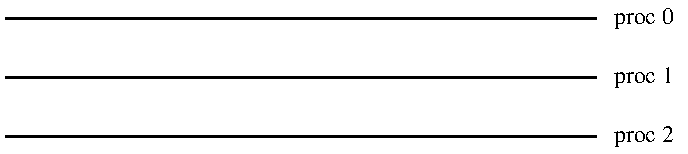
\includegraphics[width=8cm]{../../notes/04.openmp/mpi}
	\end{figure}
	\begin{itemize}
		\item In the MPI programming model, each processor has its own separate instance of the program.
		\item Hence we can consider the entire program to be one large parallel section of code.
		\item Typically parallelizing a program using MPI is done by first
			deciding on a data division between the processes, then dealing
			with the consequences of this division.
	\end{itemize}
}
\frame[label=overview4]{
\frametitle{OpenMP - program flow}
	\begin{figure}[H]
		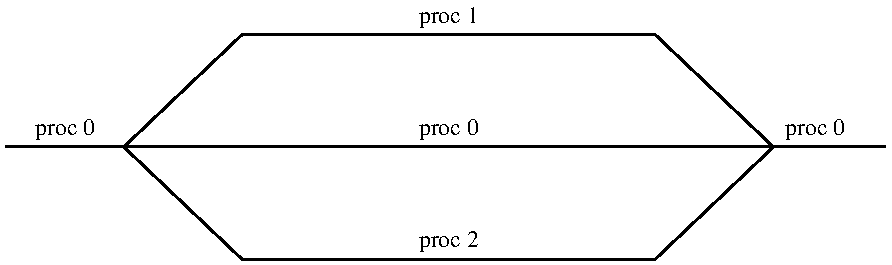
\includegraphics[width=8cm]{../../notes/04.openmp/openmp}
	\end{figure}
	\begin{itemize}
		\item OpenMP however, is based on a fork-join programming model.
		\item We only have one process.
		\item The main program flow happens on one processor, proc 0.
		\item In sections we mark as parallel using \#pragma's, the program flow
			forks into separate threads which run in parallel. Once we leave
			the parallel section, the program flow is returned to proc 0.
		\item No explicit data division is performed.
	\end{itemize}
}
\frame[label=overview2]{
\frametitle{Operations suitable for OpenMP parallelization}
	\begin{itemize}
		\item Moderately large computation intensive operations. Since thread-dispatchment
			  always has some costs attached, spawning multiple threads easily costs more
			  time than what you gain by doing the calculations in parallel if the operations
			  are too small.
		\item Decoupled problems. Since the threads are sharing resources, we have to protect
			  resources using mutual exclusion locks if several threads
			  need to read/write to the same resources concurrently. This adds code
			  complexity and in most cases severe loss of performance. OpenMP shines
			  when you are able to decouple problems in large, independent chunks.
	\end{itemize}
}
\frame[label=overview5]{
\frametitle{How to use OpenMP in your code}
	\begin{itemize}
		\item OpenMP is utilized by giving the compiler instructions through
			\emph{\#pragma} commands. Note that these instructions are \emph{NOT}
			part of the programming language itself - in contrast to \texttt{MPI}.
		\item Mainly two classes of pragmas.
		\item Either pragmas are used in combination with loop constructs.
		\item Or pragmas are used to mark sections of the code that can run in parallel.
		\item Consider the serial snippet \lstinputlisting[language=C]{../../notes/04.openmp/serial-for.c}
	\end{itemize}
}
\frame[label=overview6]{
\frametitle{OpenMP - loop example - each iteration has a fixed cost}
	\begin{itemize}
		\item We here assume that DoSomething(i); does not depend on any global resources.
	    \item To divide this loop among several threads using OpenMP you simply do \lstinputlisting[language=C]{../../notes/04.openmp/openmp-for.c}
		\item The pragma has three parts
			\begin{description}
				\item[\#pragma omp] - all openmp directives start with this.
				\item[parallel for] - instructs the compiler that we want the following
					for construct parallelized.
				\item[schedule(static)] - instructs the compiler to hand each thread approximately
					the same number of loop iterations up front.
			\end{description}
	\end{itemize}
}
\frame[label=overview7]{
\frametitle{OpenMP - loop example - each iteration has differing costs}
	\begin{itemize}
		\item Assume that each iteration of the loop has a different cost.
	    \item To divide this loop among several threads using OpenMP you do \lstinputlisting[language=C]{../../notes/04.openmp/openmp-for-dynamic.c}
		\item Note that we now use schedule(dynamic). This instructs the compiler to not divide
			  the work up front, but rather to leave one thread as a `broker'.
			  Initially each thread is assigned a single iteration. Once it finishes this iteration,
			  they ask the broker for more work. The broker keeps handing out new iterations until
			  all of them have been assigned to a thread.
	\end{itemize}
}
\frame[label=overview7.5]{
\frametitle{OpenMP - loop example - each iteration has differing costs}
	\begin{itemize}
		\item This may not work very well if there are many iterations,
			but each iteration is cheap (still different costs).
		\item Execution time is totally dominated by the negotiating with
			the broker thread.
		\item We can try to minimize this problem by specifying a \emph{chunk size};
			\lstinputlisting[language=C]{../../notes/04.openmp/openmp-for-dynamic-chunk.c}
	\end{itemize}
}
\frame[label=overview7.55]{
\frametitle{OpenMP - loop example - each iteration has differing costs}
	\begin{itemize}
		\item If we use a fixed chunk size, we may end up in a situation
			where all the remaining work is assigned to a single thread.
		\item OpenMP offers a third scheduling mode which attempts to
			minimize this problem;
			\lstinputlisting[language=C]{../../notes/04.openmp/openmp-for-guided-chunk.c}
	\end{itemize}
}
\frame[label=overview8]{
\frametitle{OpenMP - sections}
	\begin{itemize}
		\item Consider the serial snippet \lstinputlisting[language=C]{../../notes/04.openmp/serial-sections.c}
		\item We here assume that the jobs are independent and share no resources.
		\item To execute these jobs in parallel on several threads you do \lstinputlisting[language=C,basicstyle=\tiny]{../../notes/04.openmp/openmp-sections.c}
	\end{itemize}
}
\frame[label=overview10]{
\frametitle{OpenMP - syncronization}
  \begin{itemize}
    \item Since the threads share memory, we sometime have to protect resources.
    \begin{figure}[H]
            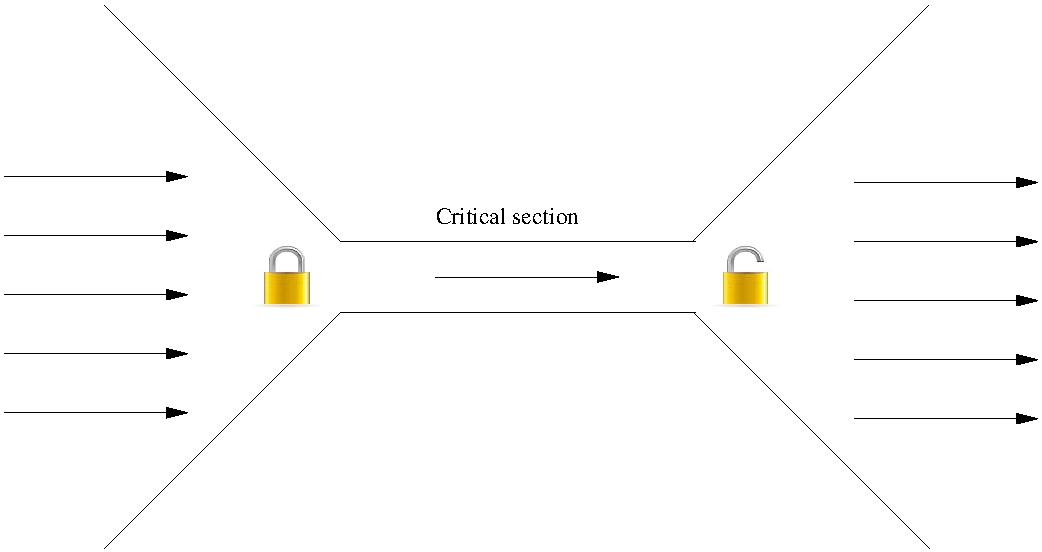
\includegraphics[width=8cm]{../../notes/04.openmp/CriticalSection}
    \end{figure}
  \end{itemize}
}
\frame[label=howto2]{
	\frametitle{OpenMP - how to enable the feature on a GNU system}
	\begin{itemize}
		\item On a GNU system you compile your C programs using
			\lstinputlisting[language=sh]{compile-gnu}
			GCC will then use reentrant functions where necessary, as well as enable OpenMP support.
		\item Note that GCC will by default silently ignore the pragmas if you compile OpenMP code without having
			OpenMP support enabled.
		\item The switches are the same for the Fortran/C++ compilers.
	\end{itemize}
}
\frame[label=howto1]{
	\frametitle{OpenMP - how to enable the feature with Intel tools}
	\begin{itemize}
		\item On a system with an Intel toolchain (like Vilje/Kongull) you compile your C programs using
			\lstinputlisting[language=sh]{compile-vilje}
		\item If you compile OpenMP code without
			the switches, the compiler will warn you that it encountered pragmas it did not understand.
			The code you end up in this case, will be exactly equivalent to a serial code.
		\item The switches are the same for the Fortran/C++ compilers.
	\end{itemize}
}
\frame[label=conclusion1]{
	\frametitle{OpenMP - conclusions}
	\begin{itemize}
		\item OpenMP offers easy exploitation of computing resources on shared memory machines.
		\item The parallel code is very close to the serial code - it usually only differs by
			some pragma's which you can tell a compiler to ignore.
		\item The fork-join programming model often is harder to grasp than the
			distributed model, in particular if several threads need to access 
			the same resources (not covered here).
		\item Best results are usually achieved if you combine OpenMP and MPI. This is also
			the model that maps the best to modern hardware, where you typically have 
			a few handfuls of cpu's sharing memory, while using more than that requires a
			distributed memory programming model.
	\end{itemize}
}
\frame[label=documentation]{
	\frametitle{OpenMP - resources}
	\begin{itemize}
		\item The official page for the OpenMP spec can be found at \emph{http://www.openmp.org}
		\item Some very instructive tutorials can be found at \emph{https://computing.llnl.gov/tutorials/openMP/}
	\end{itemize}
}
\end{document}
